\documentclass[12pt]{extarticle}
%Some packages I commonly use.
\usepackage[english]{babel}
\usepackage{graphicx}
\usepackage{framed}
\usepackage[normalem]{ulem}
\usepackage{amsmath}
\usepackage{commath}
\usepackage{amsthm}
\usepackage{amssymb}
\usepackage{amsfonts}
\usepackage{enumerate}
\usepackage[utf8]{inputenc}
\usepackage{float}
\usepackage{gensymb}
\usepackage[top=1 in,bottom=1in, left=1 in, right=1 in]{geometry}
\usepackage{multirow}
\usepackage{caption}
\usepackage{subcaption}
\usepackage{textcomp}
%A bunch of definitions that make my life easier
\newcommand{\matlab}{{\sc Matlab} }
\newcommand{\cvec}[1]{{\mathbf #1}}
\newcommand{\rvec}[1]{\vec{\mathbf #1}}
\newcommand{\ihat}{\hat{\textbf{\i}}}
\newcommand{\jhat}{\hat{\textbf{\j}}}
\newcommand{\khat}{\hat{\textbf{k}}}
\newcommand{\minor}{{\rm minor}}
\newcommand{\trace}{{\rm trace}}
\newcommand{\spn}{{\rm Span}}
\newcommand{\rem}{{\rm rem}}
\newcommand{\ran}{{\rm range}}
\newcommand{\range}{{\rm range}}
\newcommand{\mdiv}{{\rm div}}
\newcommand{\proj}{{\rm proj}}
\newcommand{\R}{\mathbb{R}}
\newcommand{\N}{\mathbb{N}}
\newcommand{\Q}{\mathbb{Q}}
\newcommand{\Z}{\mathbb{Z}}
\newcommand{\<}{\langle}
\renewcommand{\>}{\rangle}
\renewcommand{\emptyset}{\varnothing}
\newcommand{\attn}[1]{\textbf{#1}}
\theoremstyle{definition}
\newtheorem{theorem}{Theorem}
\newtheorem{corollary}{Corollary}
\newtheorem*{definition}{Definition}
\newtheorem*{example}{Example}
\newtheorem*{note}{Note}
\newtheorem{exercise}{Exercise}
\newcommand{\bproof}{\bigskip {\bf Proof. }}
\newcommand{\eproof}{\hfill\qedsymbol}
\newcommand{\Disp}{\displaystyle}
\newcommand{\qe}{\hfill\(\bigtriangledown\)}
\setlength{\columnseprule}{1 pt}
\usepackage[utf8]{inputenc}

\title{Campo Elétrico}
\author{Felipe Salvador }
\date{Abril 2019}

\begin{document}

\maketitle

\section{Introdução e motivação}


Antes de iniciar o assunto, vamos revisitar a parte de Força de Coulomb, que é a expressão de força entre 2 cargas elétricas:

\begin{equation} \label{eq:forca_coulomb}
    F_{c} = \frac{K_{0}*Q*q}{d^{2}}
\end{equation}
em que:
\begin{itemize}
    \item 
$K_{0} = \frac{1}{4\pi\epsilon_{0}}$ é uma constante chamada de \textit{Constante de Coulomb} e, para o vácuo, tem valor de: $K_{0} \simeq 8,98*10^{9} Nm^{2}/C^{2}$; 

\item
'$Q$' e '$q$' são os valores das 2 cargas, respectivamente;

\item
'$d^{2}$' é a distância entre duas cargas. Dadas as posições de $Q$ em $(x_{Q},y_{Q})$ e $q$ em $(x_{q},y_{q})$, $d^{2}$ é dado por:
\begin{equation} \label{eq:distancia}
    d^{2} = (x_{q} - x_{Q})^{2} + (y_{q} - y_{Q})^{2} 
\end{equation}

\end{itemize}
 
 Perceba que a equação (\ref{eq:forca_coulomb}) precisa das informações das 2 cargas para que nós conheçamos quão forte e para onde é a força. Fazendo uma analogia com a mecânica, em especial a Segunda Lei de Newton:
 \begin{equation} \label{eq:newton}
     \vec{F} = m\vec{a}
 \end{equation}
 Vemos que só precisamos da informação da aceleração ($\vec{a}$) para que saibamos quão forte e para onde é a força. (a massa do objeto $m$ é só um fator multiplicativo). \textbf{E se conseguirmos saber sobre quase tudo da força elétrica só com as informações de 1 carga, como na Segunda Lei de Newton?}
 
 \section{Construção do campo elétrico $\vec{E}$}
 
 É possível! E para conseguir enxergar isso, vamos voltar à equação (\ref{eq:forca_coulomb}) e reorganizá-la:
 \begin{equation} \label{eq:forca_coulomb_re}
     F_{e}= \frac{K_{0}Q}{d^{2}}*q
 \end{equation}
O que fizemos aqui foi separar o '$Q$' e o '$q$'. Agora, vamos fixar essa carga $Q$ num ponto, sabendo o seu valor, (\textit{"Vamos bater um prego para fixar a carga $Q$"}) e deixar a carga $q$ solta para colocarmos aonde quisermos. 

Como a equação (\ref{eq:forca_coulomb}) depende de $d^{2}$, descrito pela equação (\ref{eq:distancia}), e como \textit{"pregamos"} a carga $Q$ num local (ou seja, sabemos onde ela está), \textbf{a força elétrica (equação (\ref{eq:forca_coulomb})) agora só depende do valor da carga $q$ e de onde ela está (informações da carga $q$)}. E por essa mobilidade da carga $q$, nós a vamos chamar de \textbf{carga de prova ou carga teste}.

Muito bem, com isso, o primeiro fator do produto na equação se torna algo bem conhecido, pois sabemos de praticamente tudo ($K_{0}$ e $Q$). Só restaria o fator $d^{2}$, mas temos um jeito de sabermos quem é esse fator.

Para isso, vamos, para cada ponto do meu espaço $(x,y)$, calcular o $d^{2}$ por meio da equação (\ref{eq:distancia}):
\begin{equation}
    d^{2}(x,y) = (x-x_{Q})^{2} + (y-y_{Q})^{2}
\end{equation}

Com isso, sabemos \textbf{totalmente} o primeiro fator da equação (\ref{eq:forca_coulomb_re}):
\begin{equation} \label{eq:campo_eletrico}
    E = \frac{K_{0}Q}{d^{2}}
\end{equation}
E esse fator, agora, batizamos de \textbf{Campo Elétrico ($\vec{E}$)}. Portanto, podemos reescrever a equação (\ref{eq:forca_coulomb_re}) como:

\begin{equation} \label{eq:forca_campo}
    F = qE
\end{equation}
 
 Como $F$ tem unidade de \textit{Newton (N)} e carga elétrica $q$ tem unidade de \textit{Coulomb (C)}, então \textbf{o campo elétrico tem unidade de \textit{Newton por Coulomb (N/C)}}.
 
 Sabemos que força ($\vec{F}$) é uma grandeza vetorial (possui módulo, direção e sentido) e sabemos que a carga elétrica é uma grandeza escalar (só possui valor). Então, pela equação (\ref{eq:forca_campo}), \textbf{o campo elétrico (E) é uma grandeza vetorial, escrevendo-se corretamente: $\vec{E}$}.
 
 O que precisa saber dessa parte toda é que \textbf{o campo elétrico é o cara que carrega toda a informação sobre a força elétrica, a carga $q$ só contribui no cálculo do módulo da força (quão forte é).}
 
 Vocês devem estar se perguntando: \textit{Mas que raios é um 'campo'?} Na física, segundo um grande físico chamado \textit{Richard Feynman}, \textbf{campo é uma grandeza vetorial que possui um módulo, direção em sentido para cada ponto no espaço}. Ou seja, de modo mais informal, para cada ponto no espaço tem uma flecha partindo dele. A figura a seguir é a representação de um campo elétrico para uma carga no espaço:
 \begin{figure} [H]
     \centering
     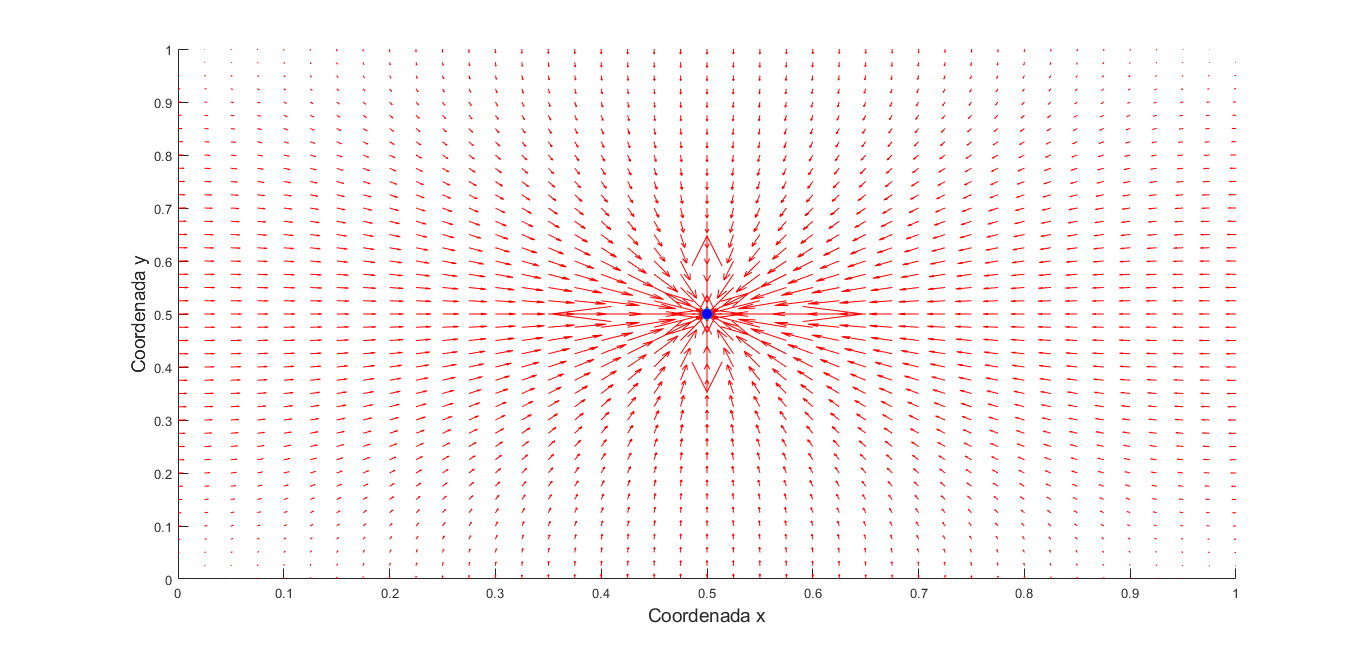
\includegraphics[width=\linewidth]{campo_eletrico.png}
     \caption{Representação do campo elétrico gerado por uma carga negativa no espaço. Há 4 setas que aparentam estar apontando no sentido oposto que das outras, mas isso ocorre porque elas começam no outro lado da carga e são tão grande que atravessam para o lado oposto}
     \label{fig:campo_eletrico}
 \end{figure}
 
 A figura acima demonstra que, colocando uma carga de prova em qualquer posição no espaço, a flecha mostra para onde ela sentiria a força elétrica e a intensidade é dada pela equação (\ref{eq:forca_campo}). 
 
\section{Superposição de campos}

Vimos que com mais de 2 cargas elétricas, a força que uma carga sofre é a soma das forças que as outras cargas fazem ela. Por exemplo, para um sistema de 4 cargas, a força sobre a carga 1 é:
\begin{equation}
    F_{1} = F_{21} + F_{31} + F_{41} 
\end{equation}
em que que $F_{21}$, por exemplo, é a força que a carga 2 exerce sobre a carga 1 e essa força é descrita por:
\begin{align*}
    F_{21} = \frac{K_{0}*q_{2}*q_{1}}{d_{21}^{2}}
\end{align*}
em que $q_{1}$ e $q_{2}$ são os valores das cargas 1 e 2; $d_{21}$ é a distância entre a carga 1 e 2.

Bem, podemos reescrever as forças pela equação (\ref{eq:forca_coulomb}), que resulta em:
\begin{align*}
    F_{1} = \frac{K_{0}*q_{2}*q_{1}}{d_{21}^{2}} + \frac{K_{0}*q_{3}*q_{1}}{d_{31}^{2}} + \frac{K_{0}*q_{4}*q_{1}}{d_{41}^{2}}
\end{align*}
Colocando em evidência $q_{1}$, temos:
\begin{align*}
    F_{1} = [\frac{K_{0}*q_{2}}{d_{21}^{2}} + \frac{K_{0}*q_{3}}{d_{31}^{2}} + \frac{K_{0}*q_{4}}{d_{41}^{2}}] q_{1}
\end{align*}
Cada parcela da soma é o campo elétrico gerado pelas cargas 2,3 e 4, segundo a equação (\ref{eq:campo_eletrico}). Logo, podemos reescrever como:

\begin{align*}
    F_{1} = [E_{2} + E_{3} + E_{4}]q_{1}
\end{align*}
Em que $E_{2}$, por exemplo, é o campo elétrico gerado pela carga 2. 
Pela equação (\ref{eq:forca_campo}), percebemos que as parcelas dos campos podem ser reescritas como:
\begin{align*}
    F_{1} = E_{1}*q_{1}
\end{align*}
Em que $E_{1}$ é:
\begin{equation} \label{eq:superpos_campo}
    E_{1} = E_{2} + E_{3} + E_{4}
\end{equation}

Isso quer dizer que \textbf{o campo elétrico que a carga 1 sente é soma (vetorial!) dos campos gerados pelas outras cargas}. A isso, damos o nome de: \textbf{Superposição de campos}.

Abaixo, podemos ver uns exemplos para um sistema de 3 cargas (2 cargas fixas que geram o campo elétrico que a carga de teste sente):
 \begin{figure} [H]
     \centering
     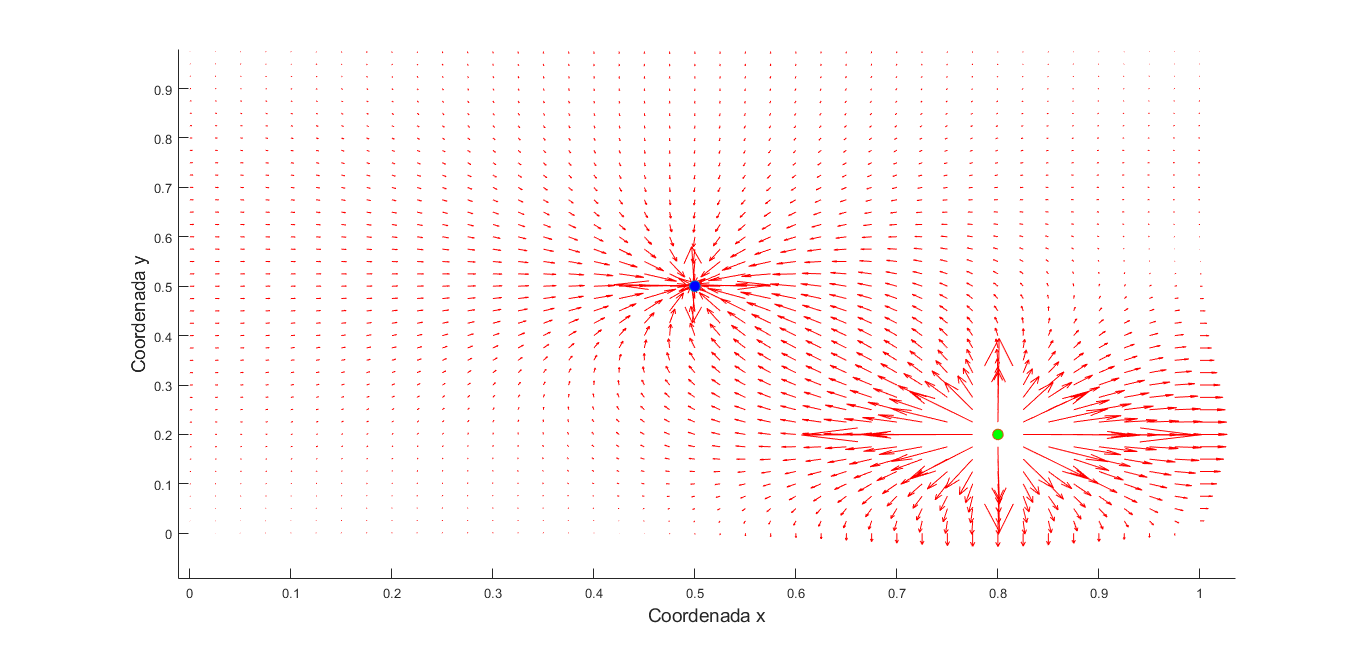
\includegraphics[width=\linewidth]{campo_eletrico_neg_pos.png}
     \caption{Representação do campo elétrico gerado por 2 cargas (1 negativa e 1 positiva). Perceba que entre as duas cargas as flechas estão apontando para uma mesma direção. Quando isso acontece, dizemos que o \textbf{campo elétrico é uniforme} nesses pontos.}
     \label{fig:campo_neg_pos}
 \end{figure}
 
 \begin{figure} [H]
     \centering
     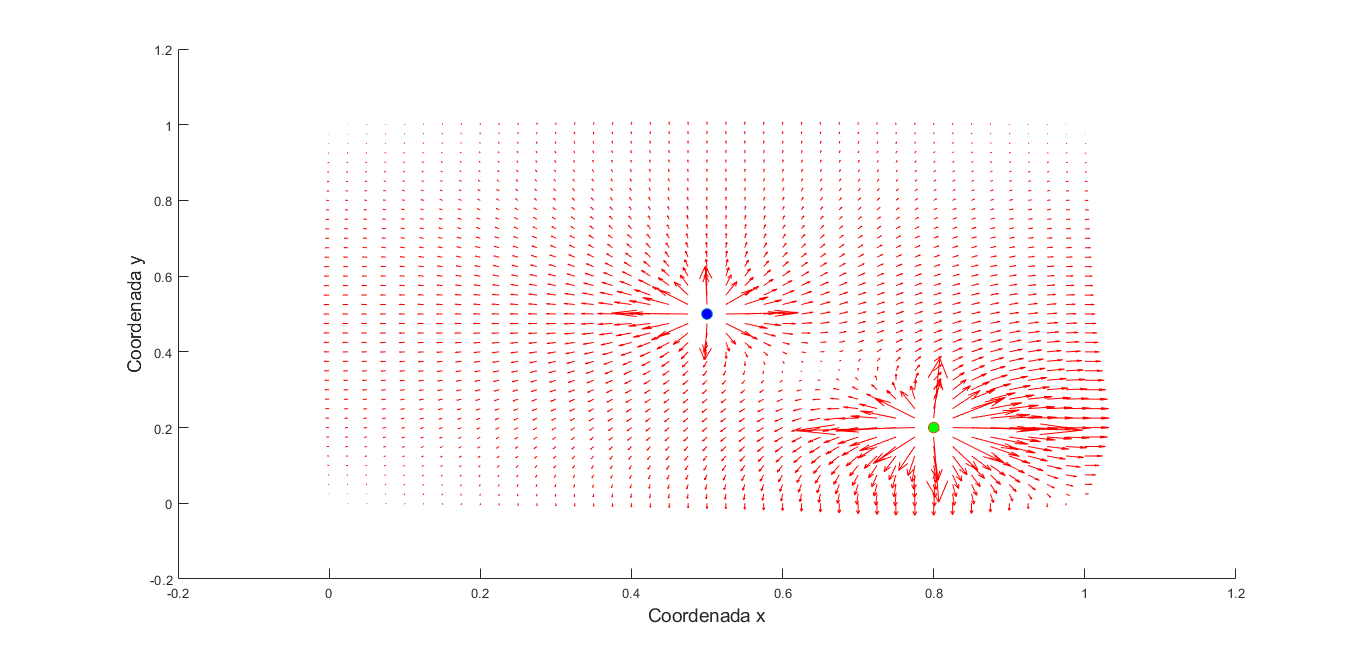
\includegraphics[width=\linewidth]{campo_eletrico_pos_pos.png}
     \caption{Representação do campo elétrico gerado por 2 cargas (2 positivas). Perceba que entre as duas cargas há pontos que não tem flechas, o que indica que, nesses pontos, \textbf{o campo elétrico é nulo}, ou seja, colocando uma carga teste ali, essa carga não iria sentir uma força. }
     \label{fig:campo_pos_pos}
 \end{figure}
 
  \begin{figure} [H]
     \centering
     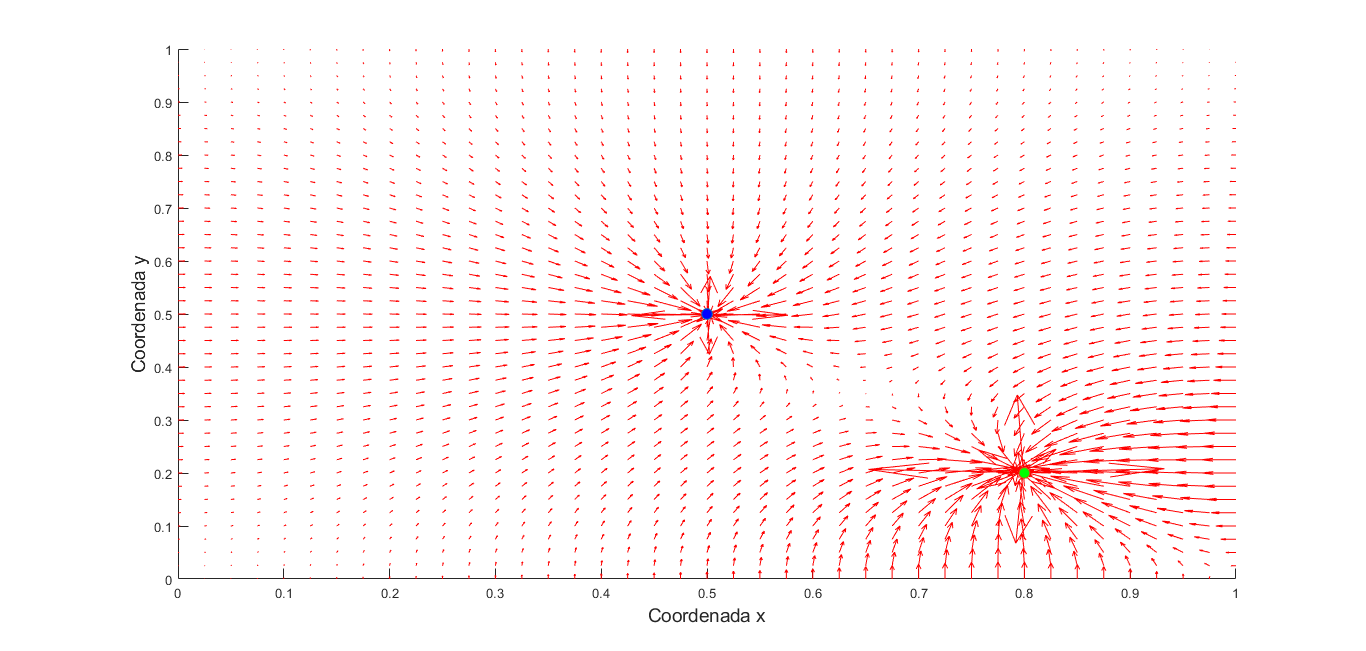
\includegraphics[width=\linewidth]{campo_eletrico_neg_neg.png}
     \caption{Representação do campo elétrico gerado por 2 cargas (as 2 negativas). Perceba que entre as duas cargas, há pontos que não tem flechas, o que indica que, nesses pontos, \textbf{o campo elétrico é nulo}, ou seja, uma carga teste nesse pontos não sente uma força elétrica.}
     \label{fig:campo_neg_neg}
 \end{figure}
 
 \section{Exemplos}
 \begin{enumerate}
     \item 
     (Mackenzie-SP): A intensidade do campo elétrico, num ponto situado a 3,0 mm de uma carga elétrica puntiforme $Q = 2,7 nC$. Calcule o campo elétrico ($E$) nesse ponto. (Dados: $K_{0} = 9*10^{9}\frac{Nm^{2}}{C^{2}}$) 
     
     Usando a equação (\ref{eq:campo_eletrico}) com os dados do problema:
     
     \begin{align*}
         E = \frac{9*10^{9}*2,7*10^{-9}}{(3*10^{-3})^{2}} \implies \mathbf{E = 2,7*10^{6} \frac{N}{C}}
     \end{align*}
     \textit{Obs: é preciso converter nC para C e mm para m}
     \item
     O campo elétrico ($E$) criado por uma carga pontual de $Q= -4 pC$, no vácuo, tem intensidade igual a $-9*10^{-1} \frac{N}{C}$. Calcule a que distância '$d$' se refere o valor desse campo. (Dados: $K_{0}= 9*10^{9} \frac{Nm^2}{C^2}$)
     
     Usando a equação (\ref{eq:campo_eletrico}) para os dados do problema:
     
     \begin{align*}
         9*10^{-1} = \frac{(-9)*10^{9}*(-4)*10^{-12}}{d^{2}}
     \end{align*}
     Isolando o $d^{2}$
     \begin{align*}
         d^{2} = \frac{36*10^{-3}}{9*10^{-1}}
     \end{align*}
     \begin{align*}
         d^{2}= 4*10^{-2} \implies \mathbf{d= 2*10^{-1}m = 0,2m = 20 cm}
     \end{align*}
     
     \item
     Duas esferas metálicas contendo as cargas $Q$ e $2Q$ estão separadas pela distância de $d=1,0 m$. Calcule o campo elétrico gerado por cada esfera no ponto médio entre as 2 esferas. \textit{Obs: deixe o seu resultado em termos de $K_{0}$ e $Q$}
     
     Como as esferas estão à $1,0m$ distante entre si, o ponto médio entre as duas esferas está a uma distância de $d' = 0.5m$. Então, pela equação (\ref{eq:campo_eletrico}), o campo elétrico gerado por uma esfera é:
     \begin{align*}
         E_{1} = \frac{K_{0}*Q}{(\frac{1}{2})^{2}}
     \end{align*}
     \begin{align*}
         E_{1} = \frac{K_{0}*Q}{\frac{1}{4}} \implies \mathbf{E_{1}=4K_{0}*Q}
     \end{align*}
     
     O campo elétrico gerado pela outra esfera é:
     \begin{align*}
         E_{2} =\frac{K_{0}*2Q}{(\frac{1}{2})^{2}}
     \end{align*}
     \begin{align*}
         E_{2} = 2\frac{K_{0}*Q}{\frac{1}{4}} \implies \mathbf{E_{2}=8K_{0}*Q}
     \end{align*}
     
     Perceba que o campo elétrico da esfera 2 é o dobro do campo elétrico da esfera 1. Então nesse ponto, uma carga teste sente uma interação maior com a esfera 2 do que com a esfera 1.


 \end{enumerate}


\end{document}
